\section{202109-1 数组推导}
\begin{itemize}
	\item 时间限制:$1.0\texttt{ s}$.
	\item 空间限制:$512.0\texttt{ MiB}$.
\end{itemize}
\subsection{题目}
\subsubsection{题目描述}
\par $A_1, A_2, \cdots, A_n$ 是一个由 $n$ 个\textbf{自然数}(即非负整数)组成的数组。在此基础上,我们用数组 $B_1 \cdots B_n$ 表示 $A$ 的前缀最大值。
$$B_i=\max\{A_1,A_2,\cdots,A_i\}$$
\par 如上所示,$B_i$ 定义为数组 $A$ 中前 $i$ 个数的最大值。
\par 根据该定义易知 $A_1=B_1$,且随着 $i$ 的增大,$B_i$ 单调不降。
\par 此外,我们用 $\text{sum}=A_1+A_2+\cdots+A_n$ 表示数组 $A$ 中 $n$ 个数的总和。
\par 现已知数组 $B$,我们想要根据 $B$ 的值来反推数组 $A$。
\par 显然,对于给定的 $B$,$A$ 的取值可能并不唯一。试计算,在数组 $A$ 所有可能的取值情况中,$\text{sum}$ 的最大值和最小值分别是多少?
\subsubsection{子任务}
\par $50\%$ 的测试数据满足数组 $B$ 单调递增,即 $0<B_1<B_2<\cdots<B_n<10^5$;
\par 全部的测试数据满足 $n\leq 100$ 且数组 $B$ 单调不降,即 $0\leq B_1\leq B_2\leq\cdots\leq B_n\leq 10^5$。
\subsection{解法 A(50 分)}
\subsubsection{原理阐释}
\par 当满足 $B$ 单调递增时,我们可以证明 $A_i=B_i(\forall i)$,过程如下。
\par 由 $B_{i+1}=\max\limits_{j=1}^{i+1}\{A_j\}$,有 $A_{i+1}\leq B_{i+1}$。
\par 假设 $A_{i+1}<B_{i+1}$,则 $B_{i+1}=\max\limits_{j=1}^{i+1}\{A_j\}=\max\{B_i,A_{i+1}\}<\max\{B_{i+1},B_{i+1}\}=B_{i+1}$,导出矛盾。从而假设不成立,我们证明了 $A_{i+1}=B_{i+1}$。
\par 综合 $A_1=B_1$,我们知道在此条件下 $A$ 的取值唯一,即为 $A_i=B_i(\forall i)$,答案即为数组 $B$ 的和。
\par 对数组 $B$ 进行求和输出,时间复杂度为 $\Theta(n)$,空间复杂度为 $\Theta(1)$。
\subsubsection{C++ 代码实现}
\lstinputlisting[
	style=C++,
	title={\bf 202109-1-subtask1.cpp}
]{202109-1-subtask1.cpp}
\subsection{解法 B(100 分)}
\subsubsection{原理阐释}
\par 与解法 A 相比,多出了 $B_{i+1}=B_i$ 的情形,此时不难看出,$A_{i+1}$ 可取 $0$ 到 $B_{i+1}$ 之间的任何值,从而由自然数加法的保序性,可以推出,欲使答案最大,需取 $A_{i+1}=B_{i+1}$,欲使得答案最小,需取 $A_{i+1}=0$。
\par 进一步整理,即得最大答案为数组 $B$ 的和,最小答案为数组 $B$ 中不同元素的和。
\par 时间复杂度为 $\Theta(n)$,空间复杂度按照去重方法可以有所不同,常见的有 $\Theta(n)$ 和 $\Theta(1)$。
\subsubsection{C++ 代码实现}
\lstinputlisting[
	style=C++,
	title={\bf 202109-1.cpp},
	tabsize=4
]{202109-1.cpp}
\subsubsection{提交结果}
\begin{figure*}[htbp]
	\centering
	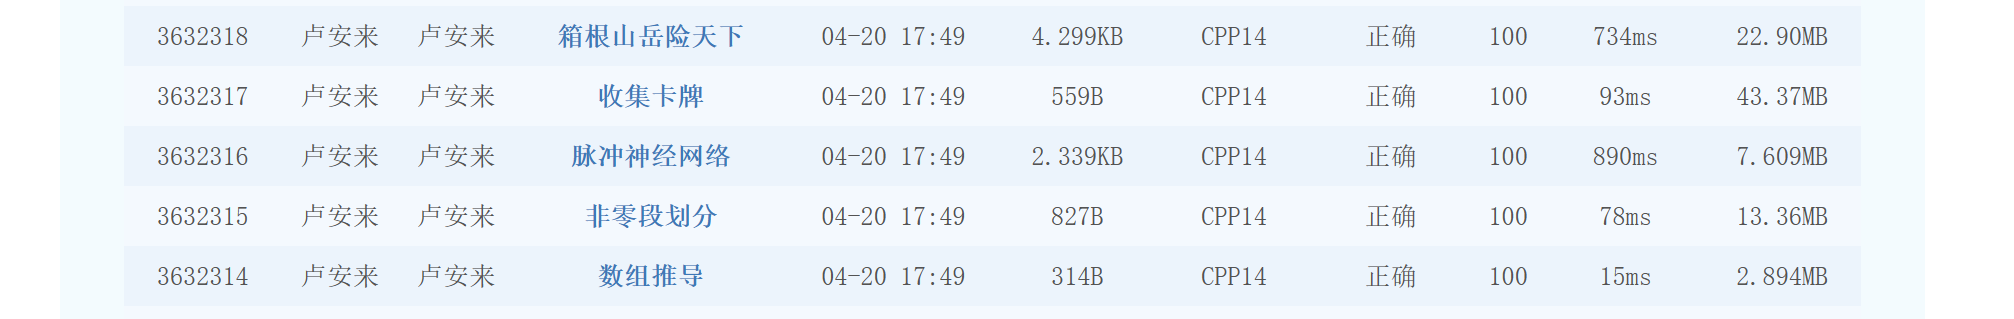
\includegraphics[width=1\textwidth]{result.png}
	\caption{提交结果}
\end{figure*}